
\documentclass[12pt]{article}

\usepackage[english]{babel}
\usepackage[utf8x]{inputenc}
\usepackage{amsmath}
\usepackage{amssymb}
\usepackage{graphicx}
\usepackage{hyperref}
\usepackage{authblk}


\title{Canonical Quantization of U(1) Chern-Simons Theory}
\author{Nilay Kumar\thanks{nk2484@columbia.edu} }
\author{Matei Ionita\thanks{mi2281@columbia.edu} }
\affil{Columbia University}


\begin{document}
\maketitle

\subsection*{Gauge symmetry}

We have seen in the previous lecture how to quantize Chern-Simon theory via path integrals. In doing this, we swept the mess of gauge invariance under the rug and focused on the explicit computation of expectation values. Today we will develop a formalism for canonical quantization, which addresses gauge invariance directly, and in the process reveals some of the features of gauge symmetry, such as the way it eliminates degrees of freedom. We will construct the Hilbert space for the quantized connections $A$ in two easy cases: when the manifold we're working on is either Euclidean space or a torus. Explicitly constructing the Hilbert space for an arbitrary manifold is beyond the scope of this lecture, but we will make some general remarks about how that procedure goes.
\\
\\
To get started, recall that quantization begins with finding the classical phase space of connections that solve the equation of motion, as well as their conjugate momenta. Then we need to find a symplectic form on this phase space - and quantization will just replace the action of the symplectic form on $p$ and $q$ with commutation relations between operators $P$ and $Q$. Recall the Chern-Simons action:
\[        S = \int_M A\wedge dA       \]
and the fact, proved in the last lecture, that flat connections $dA=0$ are the ones that extremize this action. Then we can consider our configuration space to be, to first order, the space $\{A \in \Omega_1(M): dA=0\}$. Remember, though, that observables such as Wilson loops, which depend on the integral of $A$ around some loop $\oint_{\gamma} A$, are gauge invariant, i.e. invariant under transformations $A \to A + d\theta$. It's desirable, then, to work with equivalence classes $[A] = [A + d\theta]$, in order to keep things clean and have a 1-1 correspondence between values of observables and configurations of $A$. Aesthetics apart, we saw last time that gauge invariance can actually cause path integrals to diverge, unless we get rid of it by working in the qoutient space $\{dA=0\}/d\Omega_0(M)$. From the point of view of canonical quantization, gauge invariance is bad because it makes time-evolution degenerate. If we start with a connection $A(x,0)$ at $t=0$ and time-evolve it (we'll see shortly how exactly we do that), then $A(x,t)$ is an allowed trajectory, but so is $A(x,t) + d\theta(x,t)$ for any smooth function $\theta$. But in a Hamiltonian formalism we want trajectories to be uniquely determined by initial conditions. Therefore we make a second attempt at defining a configuration space: the quotient space $\{dA=0\}/d\Omega_0(M)$, also known as $\mathcal{A}/\mathcal{G}$. In the next section we will see that we need to make yet another refinement to this definition.


\subsection*{The phase space}

It turns out that the procedure for canonically quantizing our theory will, in general, be dependent on the topological structure on which the theory is defined. So far, we have only remarked that the manifold $M$ upon which we are working is 3-dimensional. Let us now choose it to be a product $M=\Sigma\times\mathbb{R}$ where $\Sigma$ is some Riemann surface of genus $g$ (essentially just the number of holes) and the $\mathbb{R}$ component represents the time dimension. The reason we choose the ``spatial'' components of our manifold to form a Riemann surface is because they have various nice properties that we will be assuming throughout, and because such $M$'s can be ``cut-and-pasted'' to produce more general spaces. As we will see shortly, it turns out that there are no dynamics for this theory, i.e. $A(t) = A(0)$, as is to be expected from a theory that is based on topological invariants, and thus we will often conveniently forget to mention the time dimension.

Let us now write the Lagrangian in coordinates:
\begin{align*}
\mathcal{L}_{\text{CS}}&=A\wedge dA\\
&=A_i dx^i\wedge \left(dA_i\wedge dx^i\right)\\
&=A_i dx^i\wedge\left(\frac{\partial A_j}{\partial x^k} dx^k\wedge dx^j\right)\\
&=A_i\frac{\partial A_j}{\partial x^k}\left(dx^i\wedge dx^k\wedge dx^j \right)
\end{align*}
where the sums are carried out over $i,j,k=0,\ldots,2$. One rather worrying aspect of this Lagrangian is that, although there are terms containing $A_0$, there are none that contain $\partial A_0/\partial x^0$. Thus the conjugate momentum to $A_0$ is zero! It is thus impossible to quantize the $A_0$ component of our gauge field, and so we will subsequently drop it from our theory. This removes 4 terms from our Lagrangian, which allows to write it more simply as:
\begin{align*}
\mathcal{L}_\text{CS}&=A_1\frac{\partial A_2}{\partial x^0}\left(dx^1\wedge dx^0\wedge dx^2\right)+A_2\frac{\partial A_1}{\partial x^0}\left(dx^2\wedge dx^0\wedge dx^1\right)\\
&=\left(A_2\frac{\partial A_1}{\partial x^0}-A_1\frac{\partial A_2}{\partial x^0}\right)\left(dx^0\wedge dx^1\wedge dx^2\right)\\
&=\left(A_2\dot A_1-A_1\dot A_2\right)\left(dx^0\wedge dx^1\wedge dx^2\right)
\end{align*}
If we now compute the canonically conjugate momenta, we find:
\begin{align*}
\Pi_1&=\frac{\partial \mathcal{L}_\text{CS}}{\partial \dot A_1}=A_2\left(dx^0\wedge dx^1\wedge dx^2\right),\\
\Pi_2&=\frac{\partial \mathcal{L}_\text{CS}}{\partial \dot A_2}=-A_1\left(dx^0\wedge dx^1\wedge dx^2\right).
\end{align*}
Thus the conjugate momentum to one component of the field is just another! This is a very interesting situation, as our phase space of position and momenta is actually just the configuration space of $A$'s, and not twice as large! In order to formally define a phase space, we could construct a symplectic structure on $\Sigma$, but we won't go into that here. For now, simply note that the Hamiltonian of our theory is, in fact, trivial, and thus our theory has no dynamics, which justifies dropping time from our discussion throughout:
\begin{align*}
\mathcal{H}_\text{CS}&=\Pi_1 \dot A_1+\Pi_2\dot A_2\left(dx^0\wedge dx^1\wedge dx^2\right)-\mathcal{L}_\text{CS}\\
&=0.
\end{align*}


\subsection*{Quantizing on $\mathbb{R}^2$}
Before we go on with the description of Chern-Simons quantization for arbitrary manifolds, we'll talk about two simple examples that illustrate the subtleties of gauge invariance. In this section we consider the case $\Sigma = \mathbb{R}^2$. Note that, since $\mathbb{R}^2$ is simply connected, we can use Stokes' theorem to show that the integral of $A$ over any loop $\gamma$ is 0. Just let $D$ be a surface bounded by $\gamma$, then using $dA=0$ gives:
\[        \oint_{\gamma} A = \int_{D} dA = 0     \]
Therefore any Wilson loop $\exp (\oint_{\gamma} A)$ is the identity. Since the observables only take one value, we can anticipate that the phase space will also consist of only one point. This would be consistent with our desire for 1-1 correspondence between values of observables and field configurations. Let's find out how exactly does the elimination of gauge degrees of freedom get rid of all degrees of freedom. In other words, we want to show that any configuration $A$ can be gauge transformed to, say, 0.
\\
\\
Suppose we are given a configuration $(A_1, A_2)$; we want to show that there exists some function $\theta(x_1,x_2)$ such that the gauge transformed connection is 0:
\[     A_1' = A_1 - \frac{\partial}{\partial x_1} \theta(x_1, x_2)  = 0   \]
\[     A_2' = A_2 - \frac{\partial}{\partial x_2} \theta(x_1, x_2)  = 0   \]
We can simply construct $\theta$ in order to enforce the first condition for each $x_2$. Fix any $x_2$, then define:
\[  \theta(x_1, x_2) = f(x_2) + \int_0^{x_1} dy A_1(y,x_2) \]
It's easy to see that $\frac{\partial}{\partial x_1} \theta(x_1, x_2) = A_1(x_1, x_2)$ and thus $A_1'(x_1, x_2) = 0$. In the case of $A_2'$, we first show that we can enforce $A_2'(0,x_2) = 0$ by an appropriate choice of $f(x_2)$ in the above definition of $\theta$. Specifically:
\[       A_2'(0, x_2) = A_2(0, x_2) -  \frac{\partial}{\partial x_2} f(x_2) + \int_0^{x_1} dy \frac{\partial}{\partial x_2} A_1 (y,x_2)    \]
Therefore we choose:
\[      f(x_2) = \int_0^{x_2} dz \left( A_2(0,z) +  \int_0^{x_1} dy  \frac{\partial}{\partial z} A_1 (y,z) \right)   \]
And $A_2'(0, x_2) = 0$ follows. In order to extend this result for all $x_1$, recall that we are dealing with closed forms $A$, therefore:
\[    \frac{\partial A_2'}{\partial x_1} =  \frac{\partial A_1'}{\partial x_2} = 0   \]
Because $A_1' = 0$ everywhere. This shows that $A_2'$ is determined by its values at $x_1=0$, so $A_2' = 0$. Therefore the unique equivalence class in $\{dA=0\}/d\Omega_0(M)$ is $[0]$. Of course, since the phase space is trivial, so is quantizing it: the Hilbert space for Chern-Simons theory in Euclidean space is just a point.
\\
\\
Note that the above proof used the fact that $\mathbb{R}^2$ is simply connected in the way we defined $\theta$ and $f$ as integrals over domains of $\mathbb{R}^2$. If we work with a space that's not simply connected we won't be able to define line integrals everywhere, because the domain of integration will eventually cross over a hole. However, the proof can be slightly modified in order to show that any simply connected 2-manifold, and not only $\mathbb{R}^2$, has a trivial phase space. We need only pay attention to the fact that the coordinates $x_1$ and $x_2$ are defined locally and not globally (imagine the case of the sphere $S^2$), so we must work with coordinate charts.





\subsection*{The phase space on the torus $\mathbb{T}^2$}

In the previous section we saw that our Chern-Simons theory is trivial on the $\Sigma=\mathbb{R}^2$, due to $\Sigma$ being simply-connected. Let us now work with a slightly more complicated setup, where we take our universe to be the torus $\Sigma=\mathbb{T}^2$. Here it should be clear that we can no longer do away with observables so easily -- there are loops on the torus that we cannot integrate to zero via Stokes' theorem.
\begin{figure}[h]
\centering
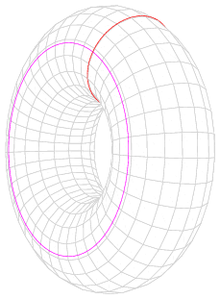
\includegraphics[width=100px]{torus.png}
\caption{The two classes of non-contractible loops on the torus.}
\label{fig:torus}
\end{figure}
In fact, there are only two ``classes'' of loops that cannot be continuously deformed to a point. These are depicted in Fig.~(\ref{fig:torus}). It is precisely such loops over which the Wilson loop is not 1, as we cannot use Stokes' theorem.
The reason we group these loops into two classes is because loops in the same class have the same value for the Wilson loop; this is easy to check by taking two loops of the same class and using Stokes' theorem to integrate $dA=0$ over the surface bounded over the surface. The difference in the integrals over the boundaries, the two loops, is thus zero. From here on, we will denote these classes as $c_1$ and $c_2$.

In this sense, given a gauge field $A$ on the torus, any Wilson loop can only take 3 possible values: 1 for a contractible loop, $\eta_1=\exp(\oint_{c_1} A)$ for a curve in $c_1$, and $\eta_2=\exp(\oint_{c_2} A)$ for a curve in $c_2$. It is quite interesting how only these values are allowed; somehow, the fact that $A$ is closed has conspired with the topology of $\Sigma$ to give us a very simple set of observables. This can be made more precise via the concept of de Rham cohomology, the study of quotient spaces such as
\begin{align*}
H^1_\text{dR}(\Sigma)=\frac{\mathcal{Z}^1(\Sigma)}{\mathcal{B}^1(\Sigma)},
\end{align*}
where $\mathcal{Z}^1(\Sigma)$ is the vector space of closed 1-forms ($dA=0$) on $\Sigma$ and $\mathcal{B}^1(\Sigma)$ is the vector space of exact 1-forms ($\omega=d\theta$) on $\Sigma$. Of course, general de Rham theory is high-powered machinery from which we will utilise only a few facts. Let's examine the simple case of $H^1_\text{dR}(\mathbb{R}^2)$ from the previous section. We showed that any $A$ closed could be taken to 0 by a gauge transformation $d\theta$. In other words, we showed that $A$ is exact. But then $H^1_\text{dR}(\mathbb{R}^2)$ must be trivial, since every closed form is exact. This is why the case of quantizing on $\mathbb{R}^2$ was so easy: our gauge symmetry asks us to only deal with equivalence classes of forms up to exact forms, but on $\mathbb{R}^2$ there is only one such equivalence class!

The case for the torus, $H^1_\text{dR}(\mathbb{T}^2)$, is not as clear; we will not compute the cohomology group here. However, by our classification of Wilson loop values above, it should be intuitive that there are really only two ``different'' types of closed forms, i.e. the two types cannot be related by an exact form. Note that each of these forms can be multiplied by a constant, and thus the cohomology group is $\mathbb{R}^2$. Although all of this may seem quite abstract, we've actually made a lot of headway: since $\mathbb{R}^2$ is the space of closed forms modulo exact forms on $\Sigma=\mathbb{T}^2$, we now know that $\mathcal{A}/\mathcal{G}=\mathbb{R}^2$!

Unfortunately, we're not quite done with computing the phase space; there is one remaining difficulty with the Wilson loops. 
At the moment, we have a one-to-one correspondence between elements of $\mathcal{A}/\mathcal{G}$ and $\eta$'s. However, the Wilson loops are sensitive to the $\eta$'s only up to the addition of $2\pi k,k\in\mathbb{Z}$ in the exponentials. Hence, we wish to quotient out this symmetry in order to finally work with ``physical'' quantities. Since we have two independent $\eta$'s, the phase space we should quantize, then, is \[\mathcal{M}=\left(\mathcal{A}/\mathcal{G}\right)/\mathbb{Z}^2=\mathbb{R}^2/\mathbb{Z}^2=\mathbb{T}^2.\]
Note that this torus is the phase space of our classical Chern-Simons theory -- not the torus $\Sigma$ that it is defined on!

To now obtain a quantum field theory, we must quantize our moduli space $\mathcal{M}$. Unfortunately, it is not at all clear how to quantize this torus; consequently, we will first quantize our old friend $\mathbb{R}^2$, and then attempt to impose certain conditions on the resulting quantum theory in order to recover a quantum theory on $\mathcal{M}$.

\end{document}




























